\documentclass{article}
\usepackage[utf8]{inputenc}
\usepackage{amsfonts}
\usepackage{amsmath}
\usepackage{amssymb}
\usepackage{amsthm}
\setlength{\parindent}{0em}
\usepackage{geometry}
\usepackage{fancyhdr}
\usepackage{graphicx}
\usepackage{graphics}
\usepackage{bbold}
\usepackage{subfig}
\usepackage{subcaption}
\usepackage{simpler-wick}
\usepackage{slashed}
\usepackage{hyperref}
\usepackage{float}
\usepackage{todonotes}
\usepackage{listings}
\usepackage{xcolor}
\pagestyle{fancy}
\fancyhf{}
\rhead{}
\lhead{}
\rfoot{Page \thepage}
 \geometry{
 a4paper,
 total={170mm,257mm},
 left=25mm,
 top=25mm,
 right=25mm,
 bottom=25mm,
 }
\definecolor{codegreen}{rgb}{0,0.6,0}
\definecolor{codegray}{rgb}{0.5,0.5,0.5}
\definecolor{codepurple}{rgb}{0.58,0,0.82}
\definecolor{backcolour}{rgb}{0.95,0.95,0.92}

\lstdefinestyle{mystyle}{
    backgroundcolor=\color{backcolour},
    commentstyle=\color{codegreen},
    keywordstyle=\color{magenta},
    numberstyle=\tiny\color{codegray},
    stringstyle=\color{codepurple},
    basicstyle=\ttfamily\footnotesize,
    breakatwhitespace=false,
    breaklines=true,
    captionpos=b,
    keepspaces=true,
    numbers=left,
    numbersep=5pt,
    showspaces=false,
    showstringspaces=false,
    showtabs=false,
    tabsize=2
}

\lstset{style=mystyle}
\makeatletter
\renewcommand{\@seccntformat}[1]{}
\makeatother
\newcommand{\ep}[0]{\varepsilon}
\newcommand{\vp}[0]{\varphi}
\newcommand{\li}[0]{\right|_{\ep = 0}}
\newcommand{\dom}[0]{\text{dom}}
\newcommand{\north}[0]{\mathcal{N}}
\newcommand{\R}[0]{\mathbb{R}}
\newcommand{\C}[0]{\mathbb{C}}
\newcommand{\ksi}[0]{\xi}
\newcommand{\T}{\mathrm{T}} % Transpose
\usepackage{braket}
\begin{document}

\title{NUMN26 - Project 1}
\author{Jimmy Gunnarsson (000513-4531) \\
        & Thomas Renström (860707-2017)}
\date{\today}
\maketitle
\newpage
\section{Task 1}
Using CVode model the elastic pendulum defined by
\[
\begin{bmatrix}
\dot{y_1}\\
\dot{y_2}\\
\dot{y_3}\\
\dot{y_4}
\end{bmatrix}
=
\begin{bmatrix}
y_3\\
y_4\\
-y_1 \lambda(y_1,y_2)\\
-y_2 \lambda(y_1,y_2) -1\\
\end{bmatrix}
\]
with
\[\lambda(y_1, y_2) = k \frac{\sqrt{y_1^2 + y_2^2}-1}{\sqrt{y_1^2 + y_2^2}}\]
where \(k\) is the spring constant.

% The simulations are represented in Figures \ref{Fig1_1}, \ref{Fig1_2} and \ref{Fig1_3}.

A elastic pendulum is a pendulum with a spring acting as the arm of a pendulum instead of a rigid body.

%With a low spring constant the spring comes to rest outstretched at \(y_1 = 0\). In fact, with \(k=0\), \(y_2 \longrightarrow -\infty\) as \(t \longrightarrow \infty\).

% At \(k=10\), we see that \(y_1\) makes a 'bounce' at the extremes, while at the higher spring constants it seems to come to a rest at the extremes. We take a close look at \(k=10\) over a longer period of time.

In Figure~\ref{Fig1_4} we see the simulation of the elastic pendulum with \(k=10\) over 50 units of time, with \(y_1\), \(y_2\), \(y_3\), and \(y_4\) being represented in blue, orange, green and red, respectively. Here we can clearly see that \(y_1\) 'bounces' when reaching its extremes. We can also see that \(y_2\) reaches different depths depending on where it is in the springs, for lack of a better word, bounce-cycle.


% \begin{figure}[H]
% \centering
% \subfloat[\(k=0\)\label{Fig1_1a}]{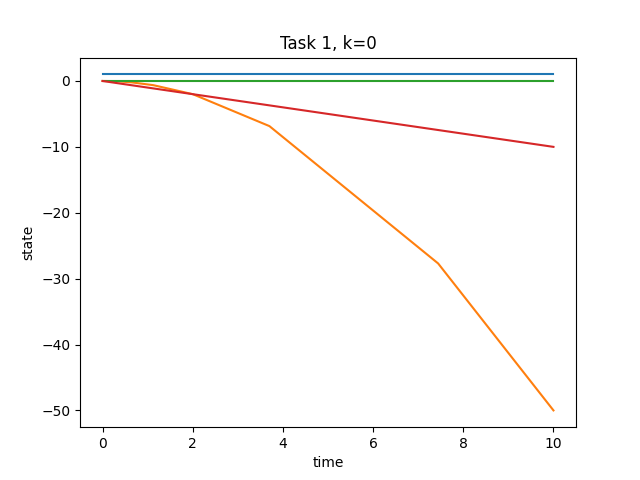
\includegraphics[width=0.50\textwidth]{Task1_figs/Figure_1_0.png}}\hfill
% \subfloat[\(k=0.1\)\label{Fig1_1b}] {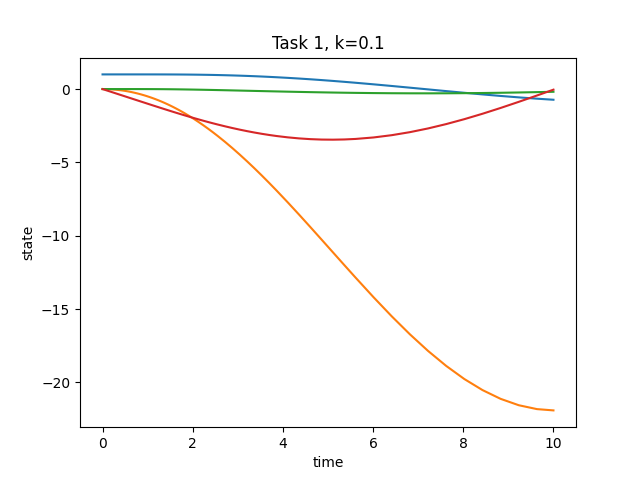
\includegraphics[width=0.50\textwidth]{Task1_figs/Figure_1_01.png}}\hfill
% \caption{Simulations using CVode.} \label{Fig1_1}
% \end{figure}

% \begin{figure}[H]
% \centering
% \subfloat[\(k=1\)\label{Fig1_2a}]{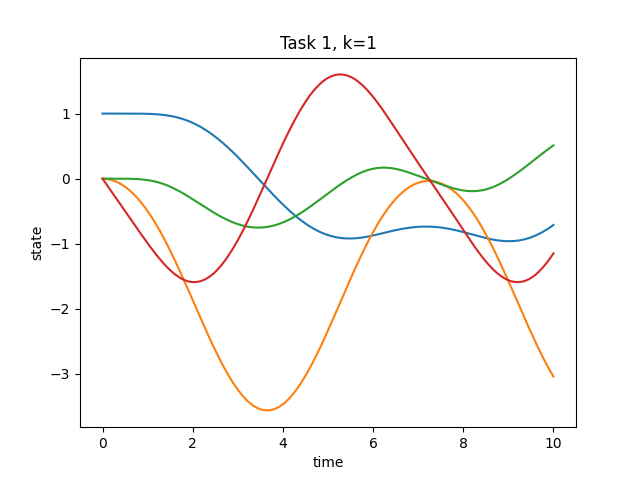
\includegraphics[width=0.50\textwidth]{Task1_figs/Figure_1_1.png}}\hfill
% \subfloat[\(k=10\)\label{Fig1_2b}] {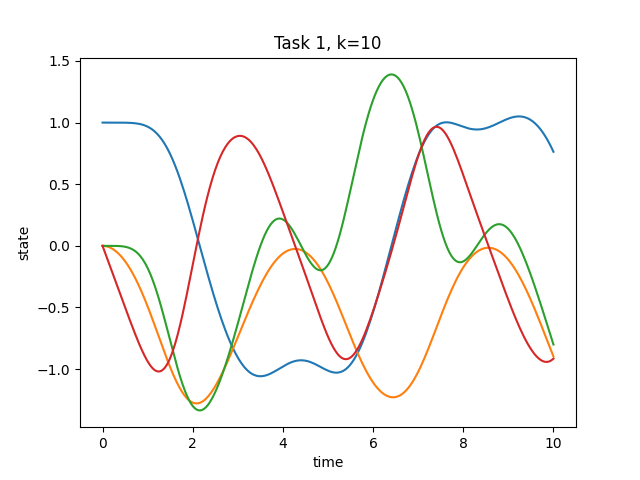
\includegraphics[width=0.50\textwidth]{Task1_figs/Figure_1_10.png}}\hfill
% \caption{Simulations using CVode.} \label{Fig1_2}
% \end{figure}

% \begin{figure}[H]
% \centering
% \subfloat[\(k=100\)\label{Fig1_3a}]{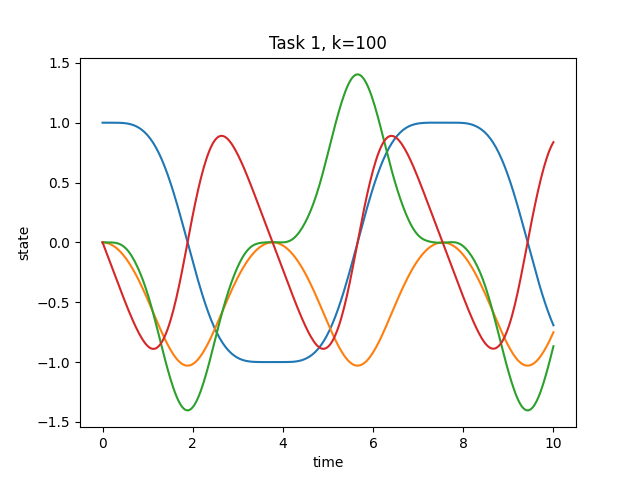
\includegraphics[width=0.50\textwidth]{Task1_figs/Figure_1_100.png}}\hfill
% \subfloat[\(k=1000\)\label{Fig1_3b}] {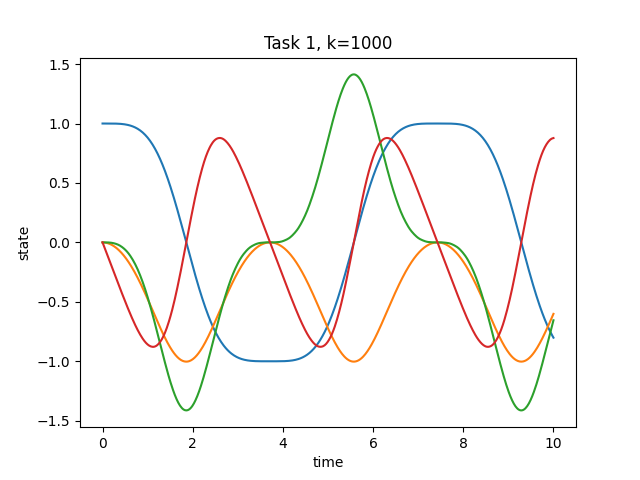
\includegraphics[width=0.50\textwidth]{Task1_figs/Figure_1_1000.png}}\hfill
% \caption{Simulations using CVode.} \label{Fig1_3}
%\end{figure}

\begin{figure}[H]
\centering
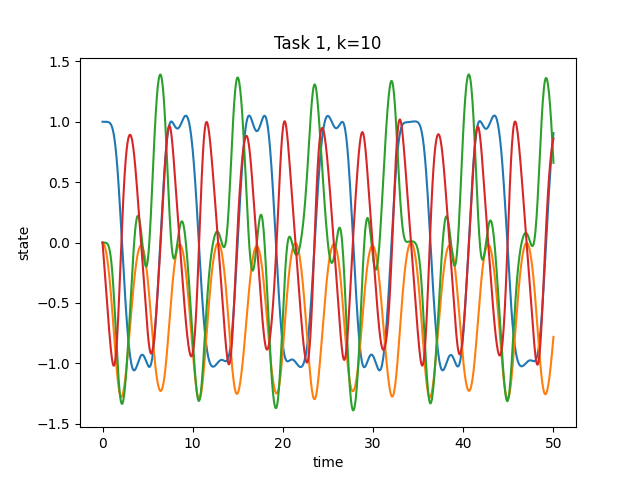
\includegraphics[width=0.80\textwidth]{Task1_figs/Figure_1_10_2.png}
\caption{Simulation using CVode with initial point \(\left[1,0,0,0\right]\).}
\label{Fig1_4}
\end{figure}

\section{Task 2}
For this task, we expand the general formulae used for BDF-2 shown in the project page. In particular, we expand it to entail BDF-3 and BDF-4. This given adaptation is supposed to be given by means of the formula usually associated with each method, and adapted, using a Newton corrector. However, we did not succeed with our Newton's method and instead used  \texttt{fsolve} for our methods.

\section{Task 3} \label{Sec:3}
Using the initial point \(y_0 = \left[2,0,0,0\right]\), we see that with an explicit Euler method the simulation seems to perform normally with \(k=1\), but at \(k=10\) it is diverging. See Figure~\ref{Fig3_1}.

\begin{figure}[H]
\centering
\subfloat[\(k=100\)\label{Fig3_3a}]{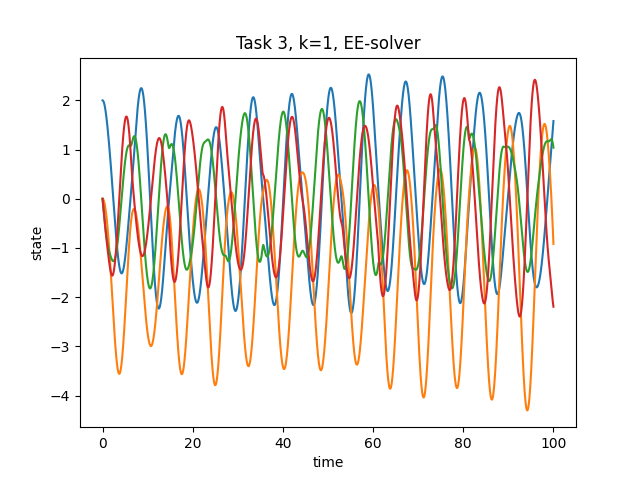
\includegraphics[width=0.50\textwidth]{Task3_figs/Figure_3_EE1.png}}\hfill
\subfloat[\(k=1000\)\label{Fig3_1b}] {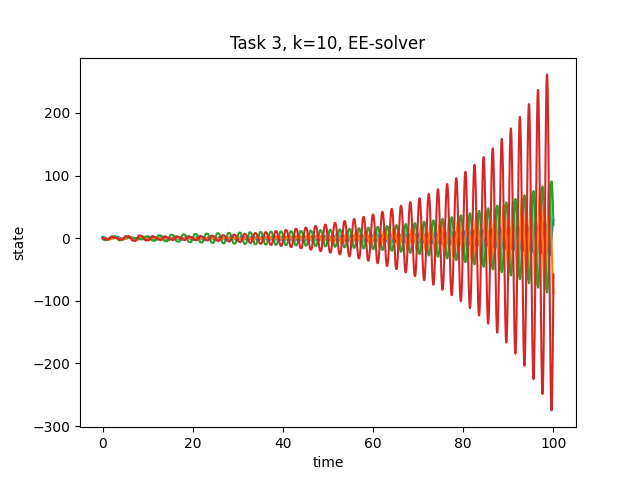
\includegraphics[width=0.50\textwidth]{Task3_figs/Figure_3_EE2.png}}\hfill
\caption{Simulations using explicit Euler with initial point \(\left[2,0,0,0\right]\).} \label{Fig3_1}
\end{figure}

For the BDF2-method with fixed point iteration we find that the method does not work for \(k=1000\) using a maximum of 100 iterations. Increasing the maximum to 1000, we find however that while the method starts high it is dampened and converges.

\begin{figure}[H]
\centering
\subfloat[\(k=100\)\label{Fig3_2a}]{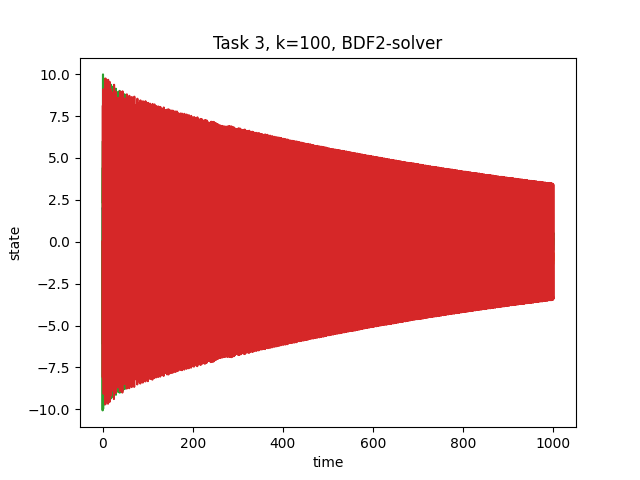
\includegraphics[width=0.50\textwidth]{Task3_figs/Figure_3_BDF2_1.png}}\hfill
\subfloat[\(k=1000\)\label{Fig3_2b}] {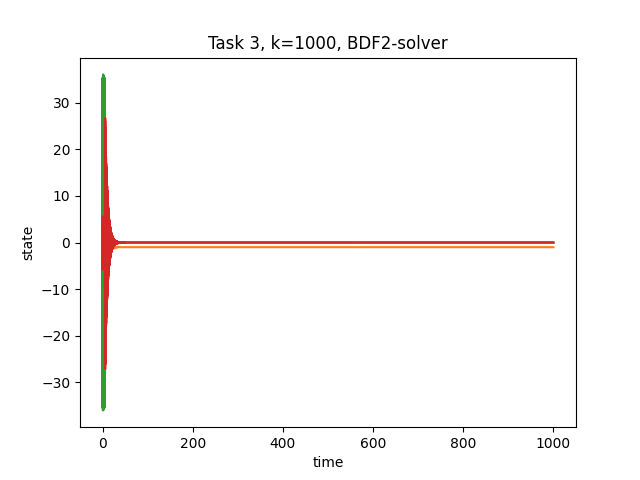
\includegraphics[width=0.50\textwidth]{Task3_figs/Figure_3_BDF2_2.png}}\hfill
\caption{Simulations using explicit BDF-2 with initial point \(\left[2,0,0,0\right]\).} \label{Fig3_2}
\end{figure}

With the BDF-3 method we can see that the simulation seems to perform normally with \(k=10\), but with \(k=100\) it exhibits the same behaviour as the explicit Euler.

\begin{figure}[H]
\centering
\subfloat[\(k=100\)\label{Fig3_3a}]{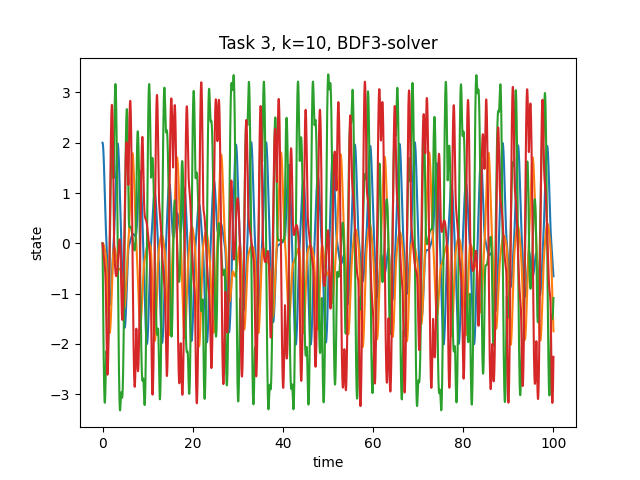
\includegraphics[width=0.50\textwidth]{Task3_figs/Figure_3_BDF3_1.png}}\hfill
\subfloat[\(k=1000\)\label{Fig3_3b}] {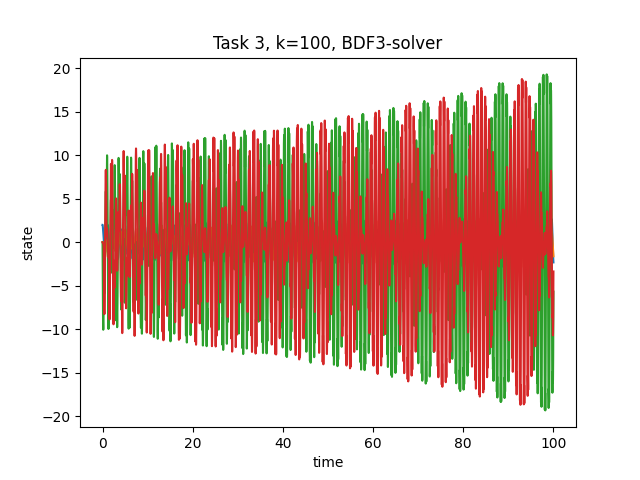
\includegraphics[width=0.50\textwidth]{Task3_figs/Figure_3_BDF3_2.png}}\hfill
\caption{Simulations using explicit BDF-3 with initial point \(\left[2,0,0,0\right]\).} \label{Fig3_3}
\end{figure}

\section{Task 4}
For this task we investigate our previous studies but with \texttt{VCODE}. Moreover, we experiment with different parameter choices included in the class, such as the discritization method, atol, rtol, and maxorder. For the other options, the default settings were used.
\begin{figure}[H]
\centering
\subfloat[Max order 2\label{Fig1_4a}]{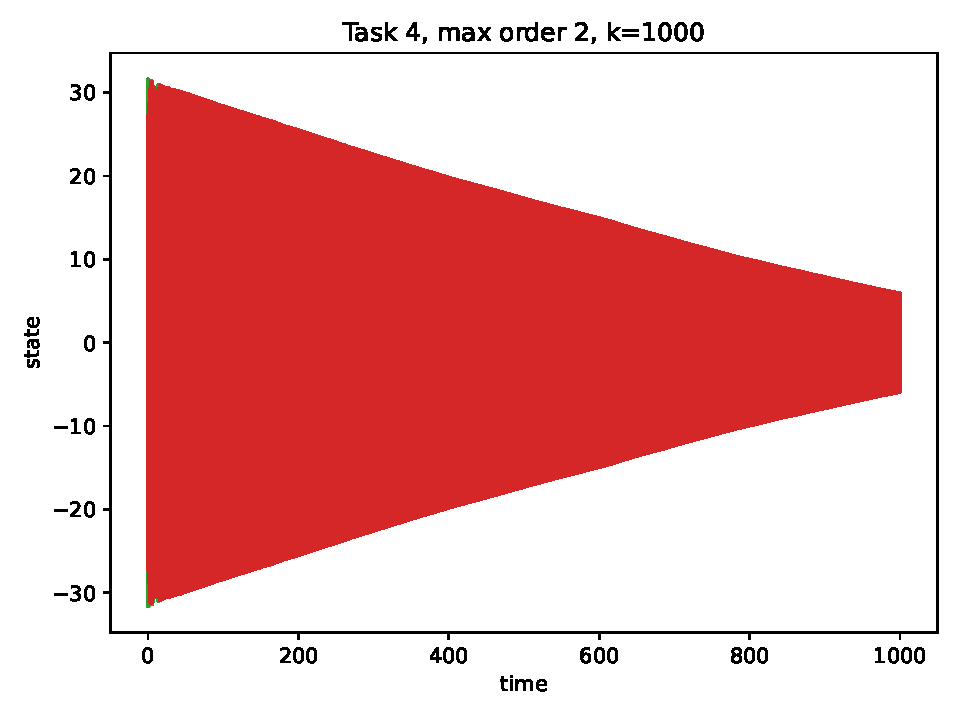
\includegraphics[width=0.50\textwidth]{Task4/Task4k1000bdf2tol-5t1000.pdf}}\hfill
\subfloat[Max order 3\label{Fig1_4b}] {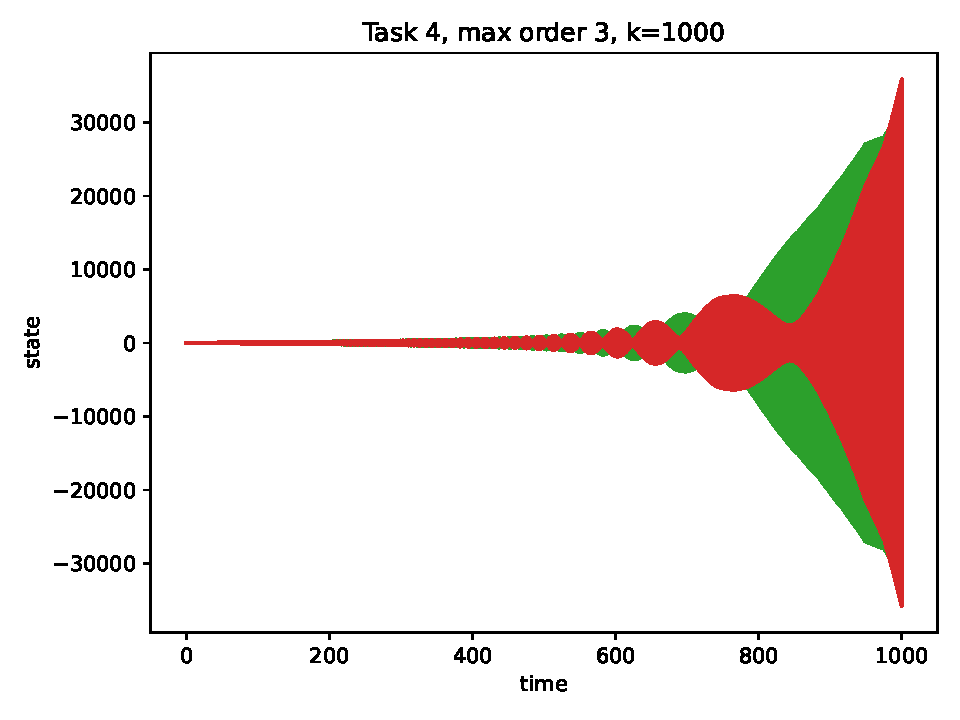
\includegraphics[width=0.50\textwidth]{Task4/Task4k1000bdf3tol-5t1000.pdf}}\hfill
\caption{BDF with different max order and atol $=$ rtol $=$ $1e-5$ with initial point \(\left[2,0,0,0\right]\).} \label{Fig4_1}
\end{figure}

\begin{figure}[H]
\centering
\subfloat[Max order 2\label{Fig2_4a}]{\includegraphics[width=0.50\textwidth]{Task4/Task4k10000bdf2tol-5t1000.pdf}}\hfill
\subfloat[Max order 3\label{Fig2_4b}] {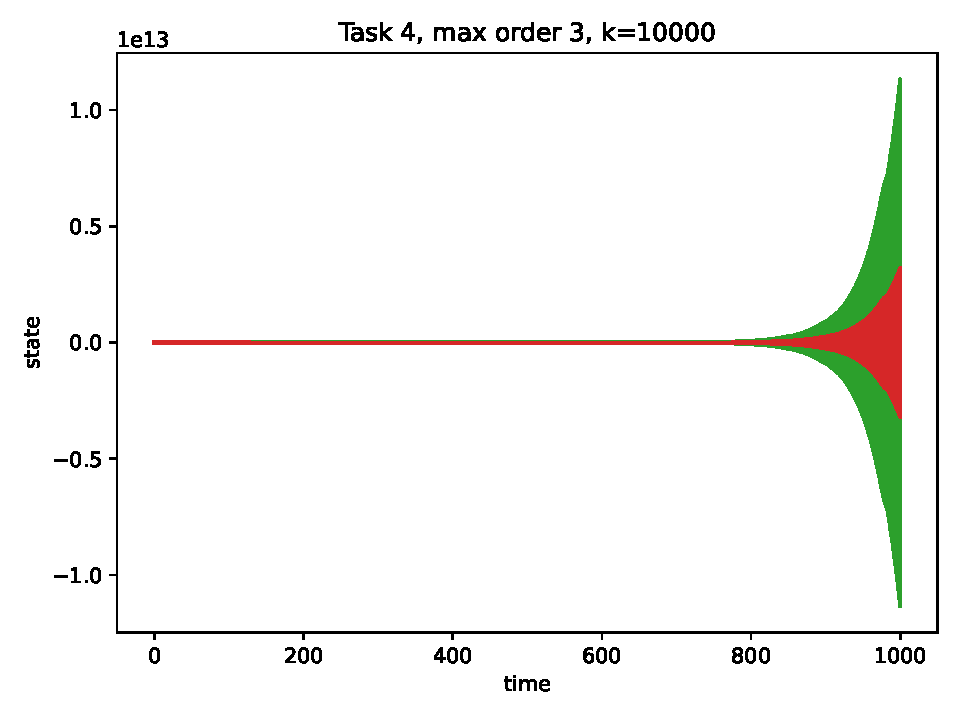
\includegraphics[width=0.50\textwidth]{Task4/Task4k10000bdf3tol-5t1000.pdf}}\hfill
\caption{BDF with different max order and atol $=$ rtol $=$ $1e-5$ with initial point \(\left[2,0,0,0\right]\).} \label{Fig4_2}
\end{figure}
Figures \ref{Fig4_1} and \ref{Fig4_2} showcase that BDF of maximal order $2$ and $3$ with the given tolerances would not yield a conserved system over long periods of time. Such is shown as the spring system is not norm-conserving as the oscillations either diverge to infinity (for maximal order of 3), or converge to a stationary point (for maximal order of 2). We can relay this discussion to the previous investigation in Section \ref{Sec:3}.

\begin{figure}[H]
\centering
\subfloat[Max order 2\label{Fig3_4a}]{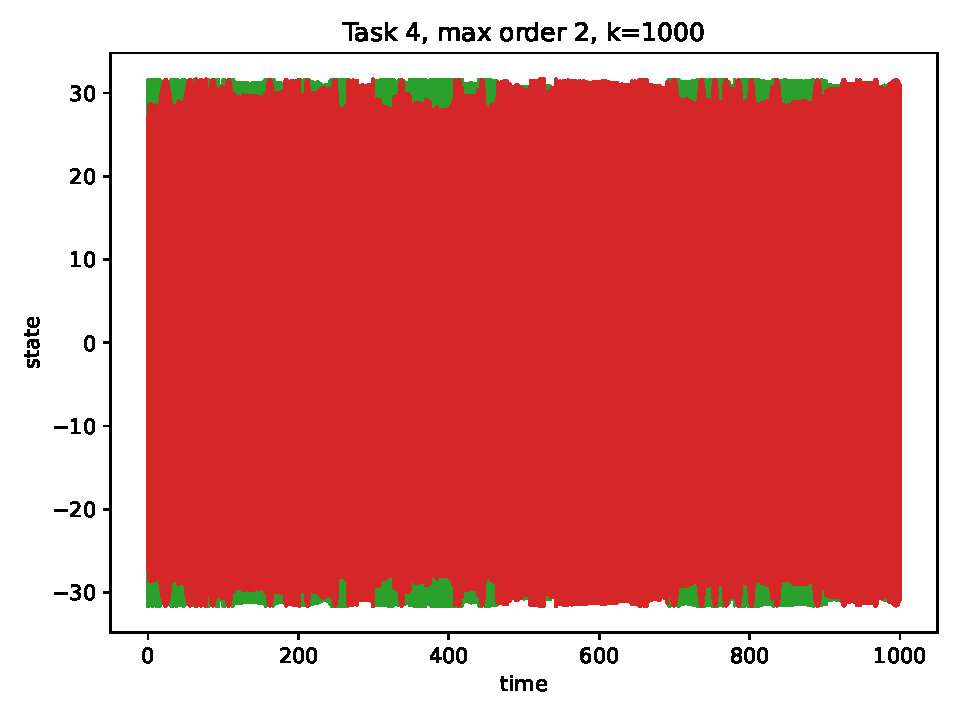
\includegraphics[width=0.50\textwidth]{Task4/Task4k1000adam2tol-5t1000.pdf}}\hfill
\subfloat[Max order 3\label{Fig3_4b}] {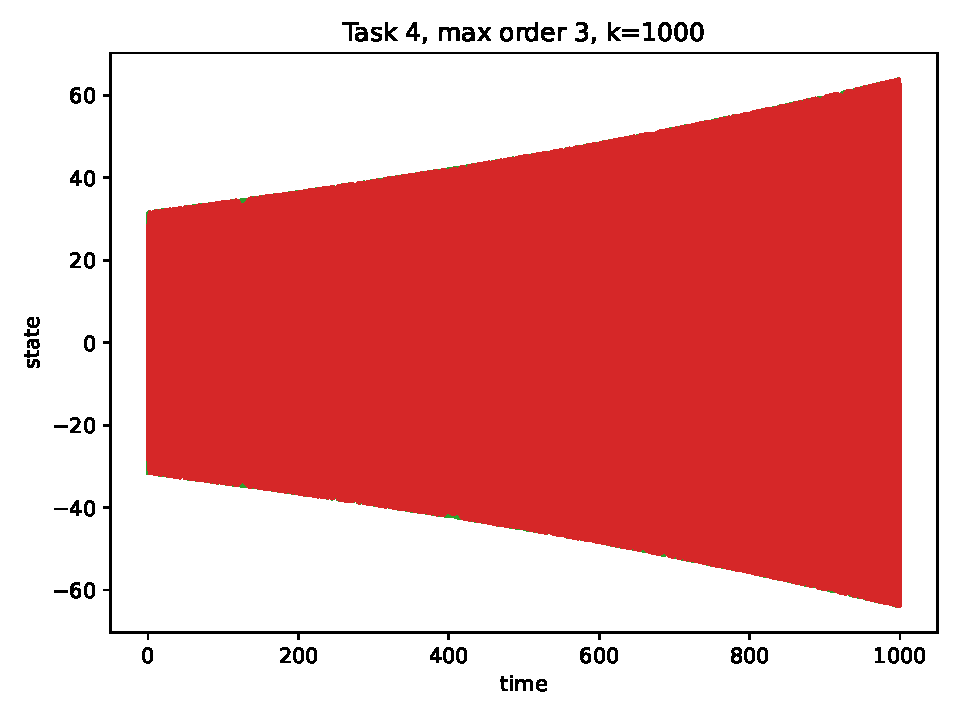
\includegraphics[width=0.50\textwidth]{Task4/Task4k1000adam3tol-5t1000.pdf}}\hfill
\caption{Adams with different max order and atol $=$ rtol $=$ $1e-5$ with initial point \(\left[2,0,0,0\right]\).} \label{Fig4_3}
\end{figure}

\begin{figure}[H]
\centering
\subfloat[atol $=$ rtol $=$ $1e-4$\label{Fig4_4a}]{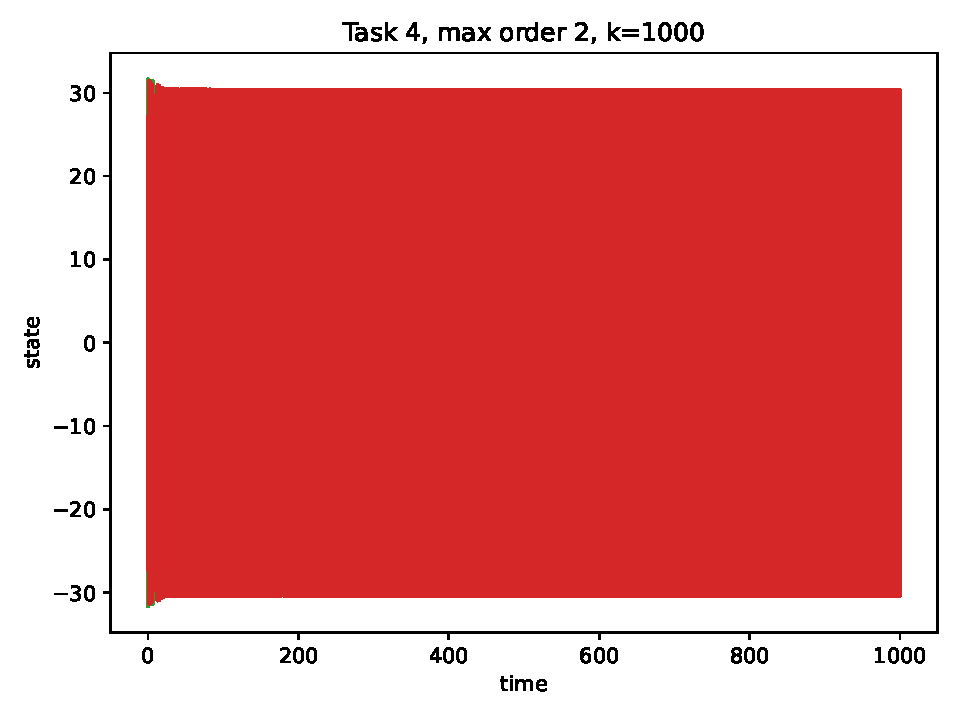
\includegraphics[width=0.50\textwidth]{Task4/Task4k1000adam2tol-4t1000.pdf}}\hfill
\subfloat[atol $=$ rtol $=$ $1e-3$\label{Fig4_4b}] {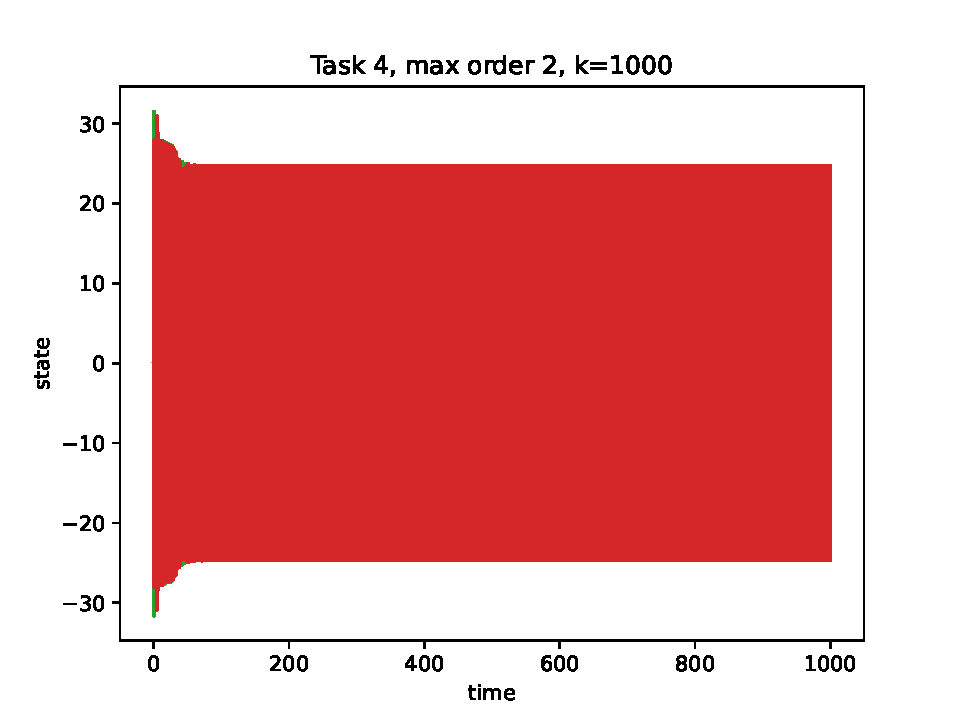
\includegraphics[width=0.50\textwidth]{Task4/Task4k1000adam2tol-3t1000.pdf}}\hfill
\caption{Adams with different tolerances with initial point \(\left[2,0,0,0\right]\).} \label{Fig4_4}
\end{figure}
We then draw our attention to investigating the behaviour of Adam's method. Figure \ref{Fig4_3} showcases the stability of different max orders. It is clear that when the max order is $2$, then we obtain a stable solution, while we obtain an unstable solution when the max order is $3$. However, we can note that by comparing Figures \ref{Fig1_4b} and \ref{Fig3_4b} that Adam's appear more stable than the BDF method, and that oscillations are more variant for large time scales with BDF. \\

We then investigate the dependency on the tolerances for Figures \ref{Fig3_4a}, \ref{Fig4_4a}, and \ref{Fig4_4b}. It is clear that Adams is stable for max order $2$ for large time scales. However, when we investigate the early time behaviour we notice a spike for Figures \ref{Fig4_4a}, and \ref{Fig4_4b} compared to Figure \ref{Fig3_4a}. This can be explained by the fact that the method becomes stable after corrections for the small tolerance -- before ultimately becomes stable. In practical use, however, the chosen tolerance studied for Adams of max order $2$ is the one that we investigated in Figure \ref{Fig4_4a}, and as such, is optimal for practical purposes. \\


\section{Task 5}
We investigated the Assimulo package for different configurations of problems. From the methods provided in this package, we build our own BDF-3 and BDF-4 solvers as children classes to \texttt{Explicit$\_$ODE} from Assimulo to simulate a spring problem. We verified the set-up by investigating the simulation using \texttt{CVODE}. After such was performed, we did a stability study of the problem by changing the spring constant $k$ and iterating over different periods of time. \\

\noindent Finally, we replicated parts of our experiment with \texttt{CVODE} from Assimulo using different options from the simulation class. By doing such, we were able to investigate the differences in application and adaptations dependent on parameter options.

\appendix
\newpage
\section{Appendix: Code}
To reproduce the results that we have obtained, run the following code for the studies solvers. The spring constant $k$ can be initiated and then following through by defining the problem. Then, by using the corresponding solver, a simulation of the solution can be generated. Plotting can then be conducted through the simulation method.
\begin{lstlisting}[language=python]
class BDF_general(Explicit_ODE):
    maxsteps = 500
    maxit = 100
    tol = 1.e-8

    def __init__(self, problem, degree):
        Explicit_ODE.__init__(self, problem)
        self.degree = degree

        # Solver options
        self.options["h"] = 0.01
        # Statistics
        self.statistics["nsteps"] = 0
        self.statistics["nfcns"] = 0

    def _set_h(self, h):
        self.options["h"] = float(h)

    def _get_h(self):
        return self.options["h"]

    def integrate(self, t0, y0, tf, opts):
        h = min(self._get_h(), np.abs(tf-t0))
        t_list = [t0]
        y_list = [y0]

        self.statistics["nsteps"] += 1
        t, y = self.EEstep(t0, y0, h)
        t_list.append(t)
        y_list.append(y)
        h = min(self._get_h(), np.abs(tf-t0))

        for i in range(1, self.maxsteps):
            if t >= tf:
                break
            self.statistics["nsteps"] += 1
            t, y = self.BDFstep_general(t, y_list[-self.degree:][::-1], h)
            t_list.append(t)
            y_list.append(y)
            h = min(self._get_h(), np.abs(tf-t))

        return ID_PY_OK, t_list, y_list

    def EEstep(self, t_n, y_n, h):
        self.statistics["nfcns"] += 1
        return t_n + h, y_n + h*self.problem.rhs(t_n, y_n)

    def BDFstep_general(self, t_n, Y, h):
        coeffs = [[1, 1],
                  [4/3, -1/3, 2/3],
                  [18/11, -9/11, 2/11, 6/11],
                  [48/25, -36/25, 16/25, -3/25, 12/25],
                  [300/137, -300/137, 200/137, -75/137, 12/137, 60/137],
                  [360/147, -450/147, 400/147, -225/147, 72/147, -10/147, 60/147]]
        return self.BDFstep_general_internal(t_n, Y, coeffs[len(Y)-1], h)

    def BDFstep_general_internal(self, t_n, Y, coeffs, h):
        static_terms = coeffs[0] * Y[0]
        for i in range(1, len(Y)):
            static_terms += coeffs[i] * Y[i]

        # Predictor
        t_np1 = t_n + h
        y_np1_i = Y[0]
        for i in range(self.maxit):
            # BDF Evaluator
            y_np1_temp = static_terms + coeffs[-1]*h*self.problem.rhs(t_np1, y_np1_i)
            self.statistics["nfcns"] += 1
            # FPI Corrector
            y_np1_ip1 = y_np1_temp

            if(np.linalg.norm(y_np1_ip1-y_np1_i)) < self.tol:
                return t_np1, y_np1_ip1
            y_np1_i = y_np1_ip1
        else:
            raise Explicit_ODE_Exception(f"Corrector could not converge within {i} iterations")


class BDF_general_newton(BDF_general):
    maxsteps = 500
    maxit = 100
    tol = 1.e-8

    def __init__(self, problem, degree):
        Explicit_ODE.__init__(self, problem)
        self.degree = degree
        # Solver options
        self.options["h"] = 0.01
        # Statistics
        self.statistics["nsteps"] = 0
        self.statistics["nfcns"] = 0

    def BDFstep_general_internal(self, t_n, Y, coeffs, h):
        static_terms = coeffs[0] * Y[0]
        for i in range(1, len(Y)):
            static_terms += coeffs[i] * Y[i]

        # Predictor
        t_np1 = t_n + h
        y_np1_i = Y[0]
        Newton_func = lambda x: (static_terms + coeffs[-1]*h*self.problem.rhs(t_np1, x)) - x
        y_np1_ip1, info = opt.fsolve(Newton_func, y_np1_i, xtol=self.tol, full_output=True)[:2]
        self.statistics["nfcns"] += info["nfev"]
        return t_np1, y_np1_ip1


class BDF_2(BDF_general):
    def __init__(self, problem):
        BDF_general.__init__(self, problem, 2)


class BDF_3(BDF_general):
    def __init__(self, problem):
        BDF_general.__init__(self, problem, 3)


class BDF_4(BDF_general):
    def __init__(self, problem):
        BDF_general.__init__(self, problem, 4)


class BDF_3_newton(BDF_general_newton):
    def __init__(self, problem):
        BDF_general.__init__(self, problem, 3)


class BDF_4_newton(BDF_general_newton):
    def __init__(self, problem):
        BDF_general.__init__(self, problem, 4)
\end{lstlisting}
\end{document}
